\documentclass[svgnames,dvipsnames,hyperref={bookmarks=false},usepdftitle=false]{beamer}
\usetheme{scalasphere}
\usepackage{tikz}
\usetikzlibrary[arrows.meta]

\title{Scala.meta semantic API}
\author{Eugene Burmako (\href{https://twitter.com/xeno_by}{@xeno{\textunderscore}by})}
\institute{
\includegraphics[height=1cm]{twitter.png}}
\date{2 March 2017}
\hypersetup{pdfauthor={Eugene Burmako},pdftitle={Scala.meta semantic API}}

\begin{document}

\titleframe

\sectionframe{What is scala.meta?}

\begin{frame}{scala.meta is a cutting edge research}
\vskip20pt
\begin{center}
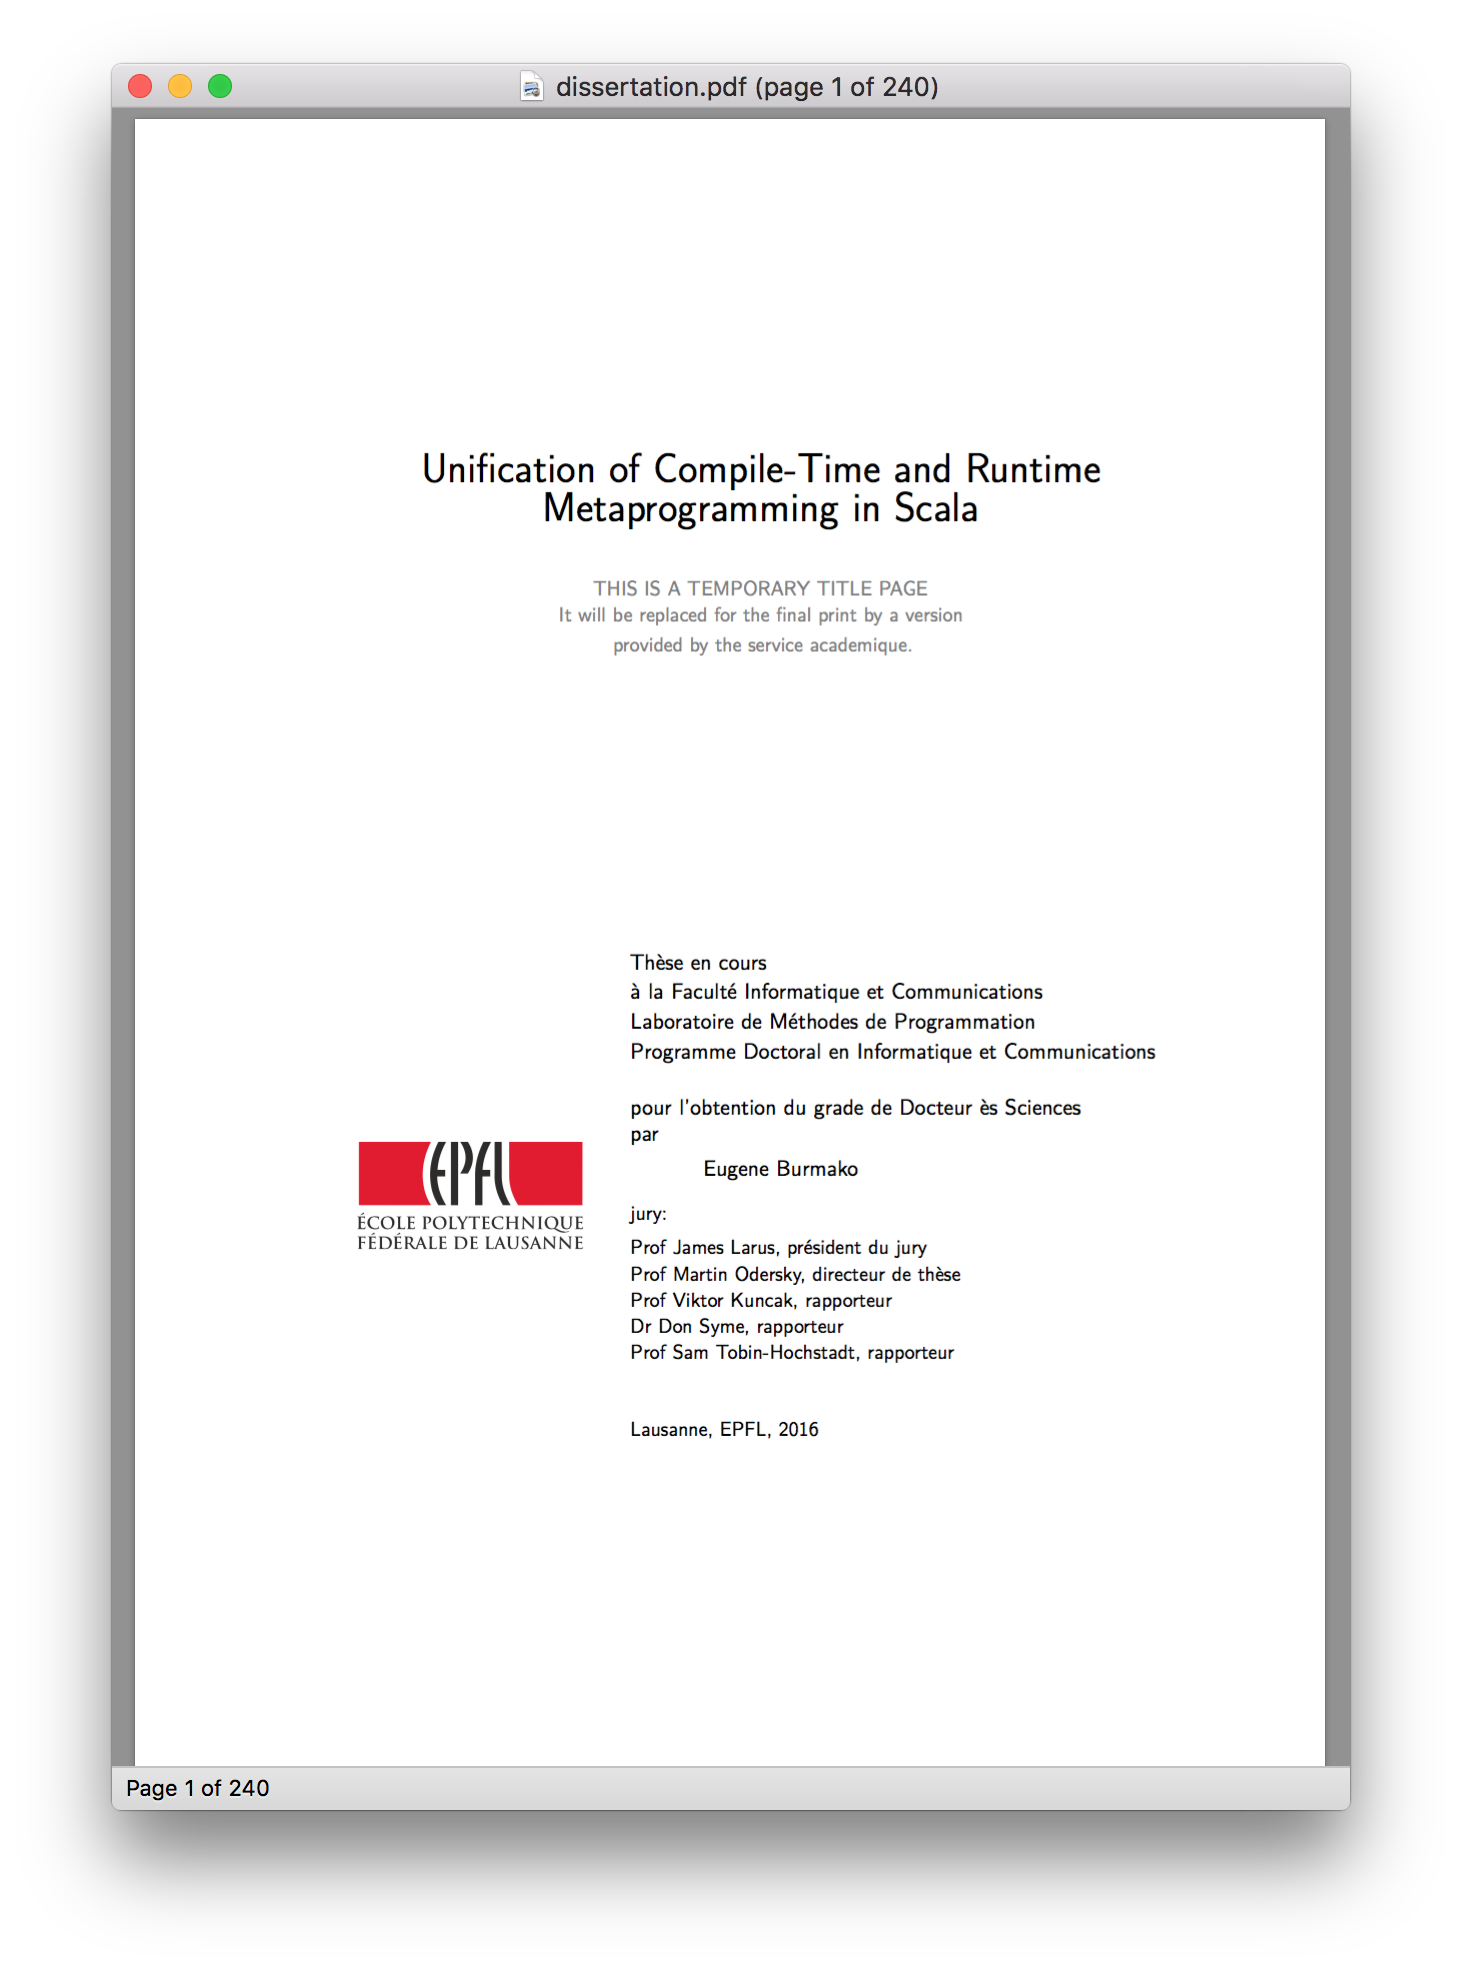
\includegraphics[height=8.5cm]{is-a-cutting-edge-research.png}
\end{center}
\end{frame}

\begin{frame}{scala.meta is officially endorsed (EPFL)}
\vskip20pt
\begin{center}
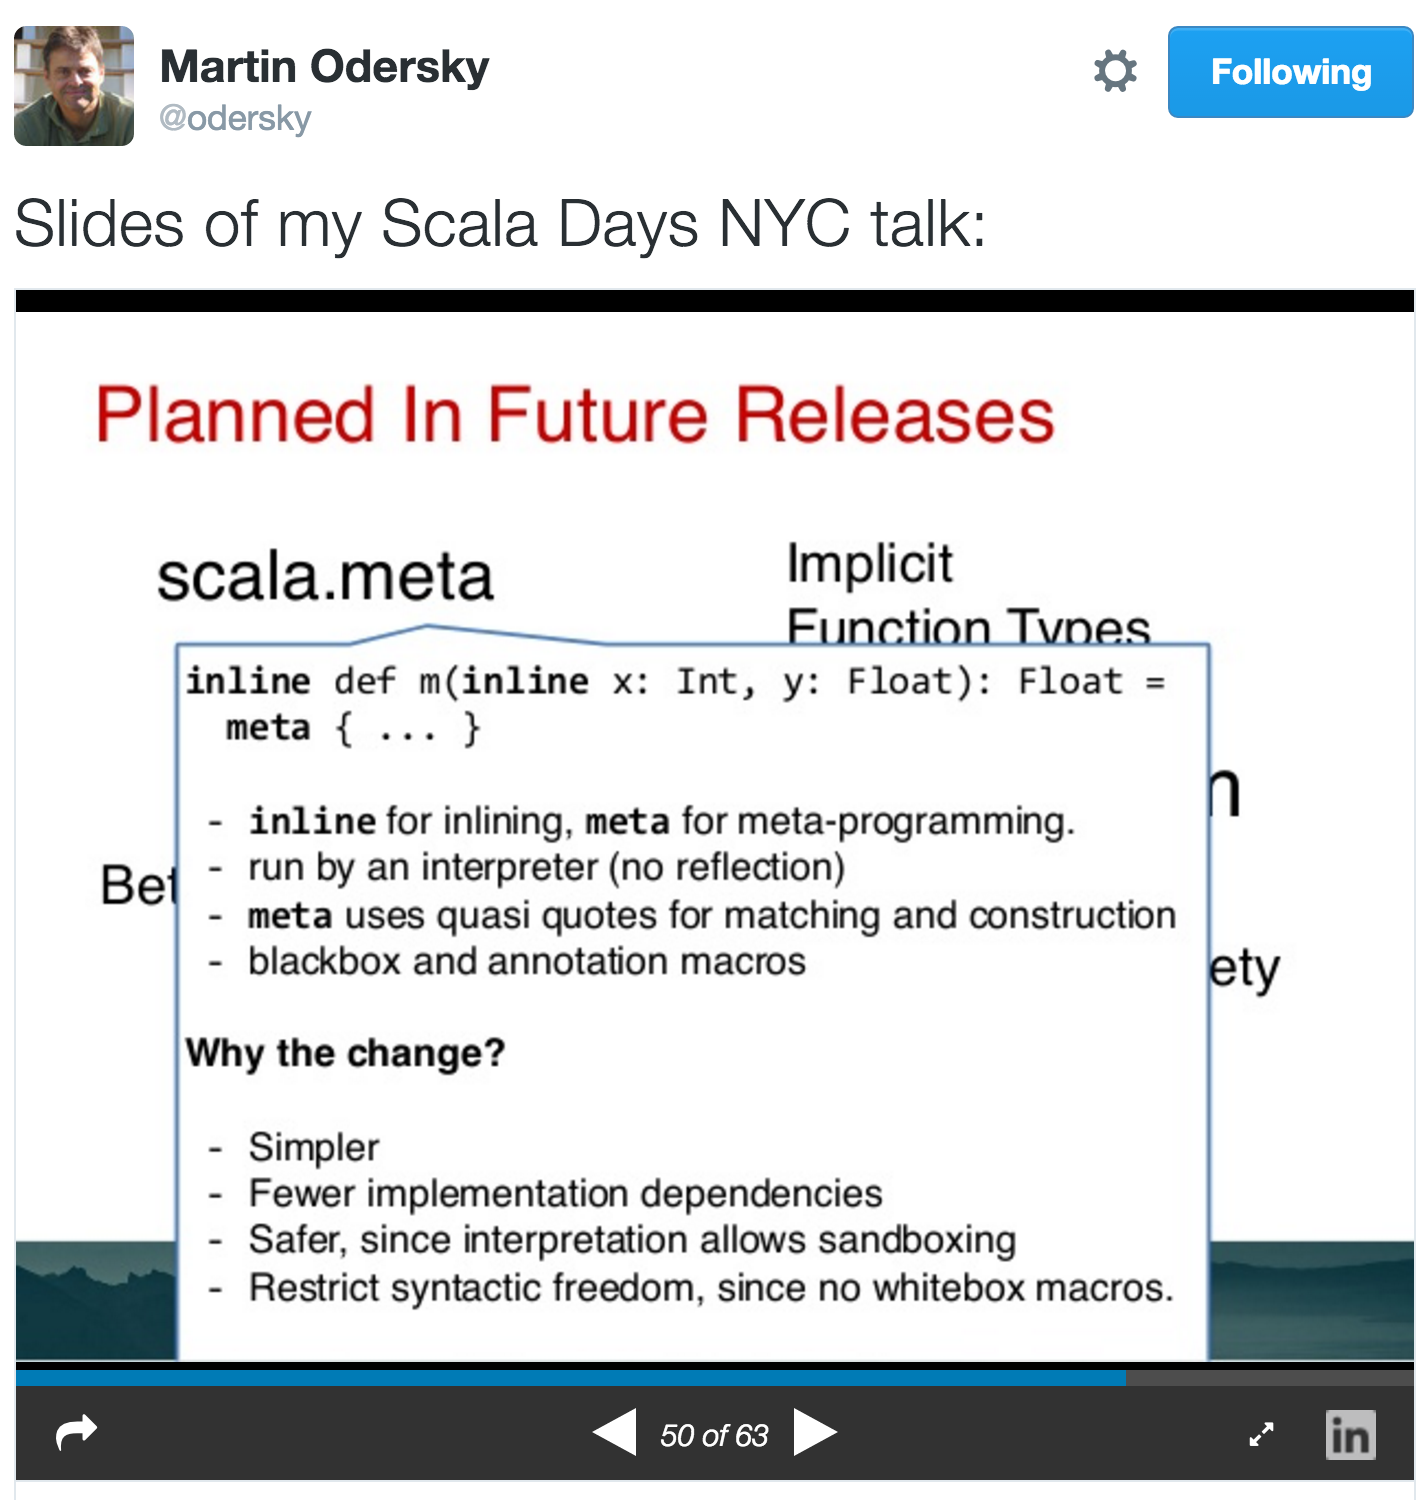
\includegraphics[height=7.5cm]{is-officially-endorsed-1.png}
\end{center}
\end{frame}

\begin{frame}{scala.meta is officially endorsed (Twitter)}
\vskip20pt
\begin{center}

\includegraphics[height=7.5cm]{is-officially-endorsed-2.png}
\end{center}
\end{frame}

\begin{frame}{scala.meta is officially endorsed (Scala Center)}
\vskip20pt
\begin{center}

\includegraphics[height=6.25cm]{is-officially-endorsed-3.png}
\end{center}
\end{frame}

% \begin{frame}{scala.meta is an active project}
% \begin{center}
% 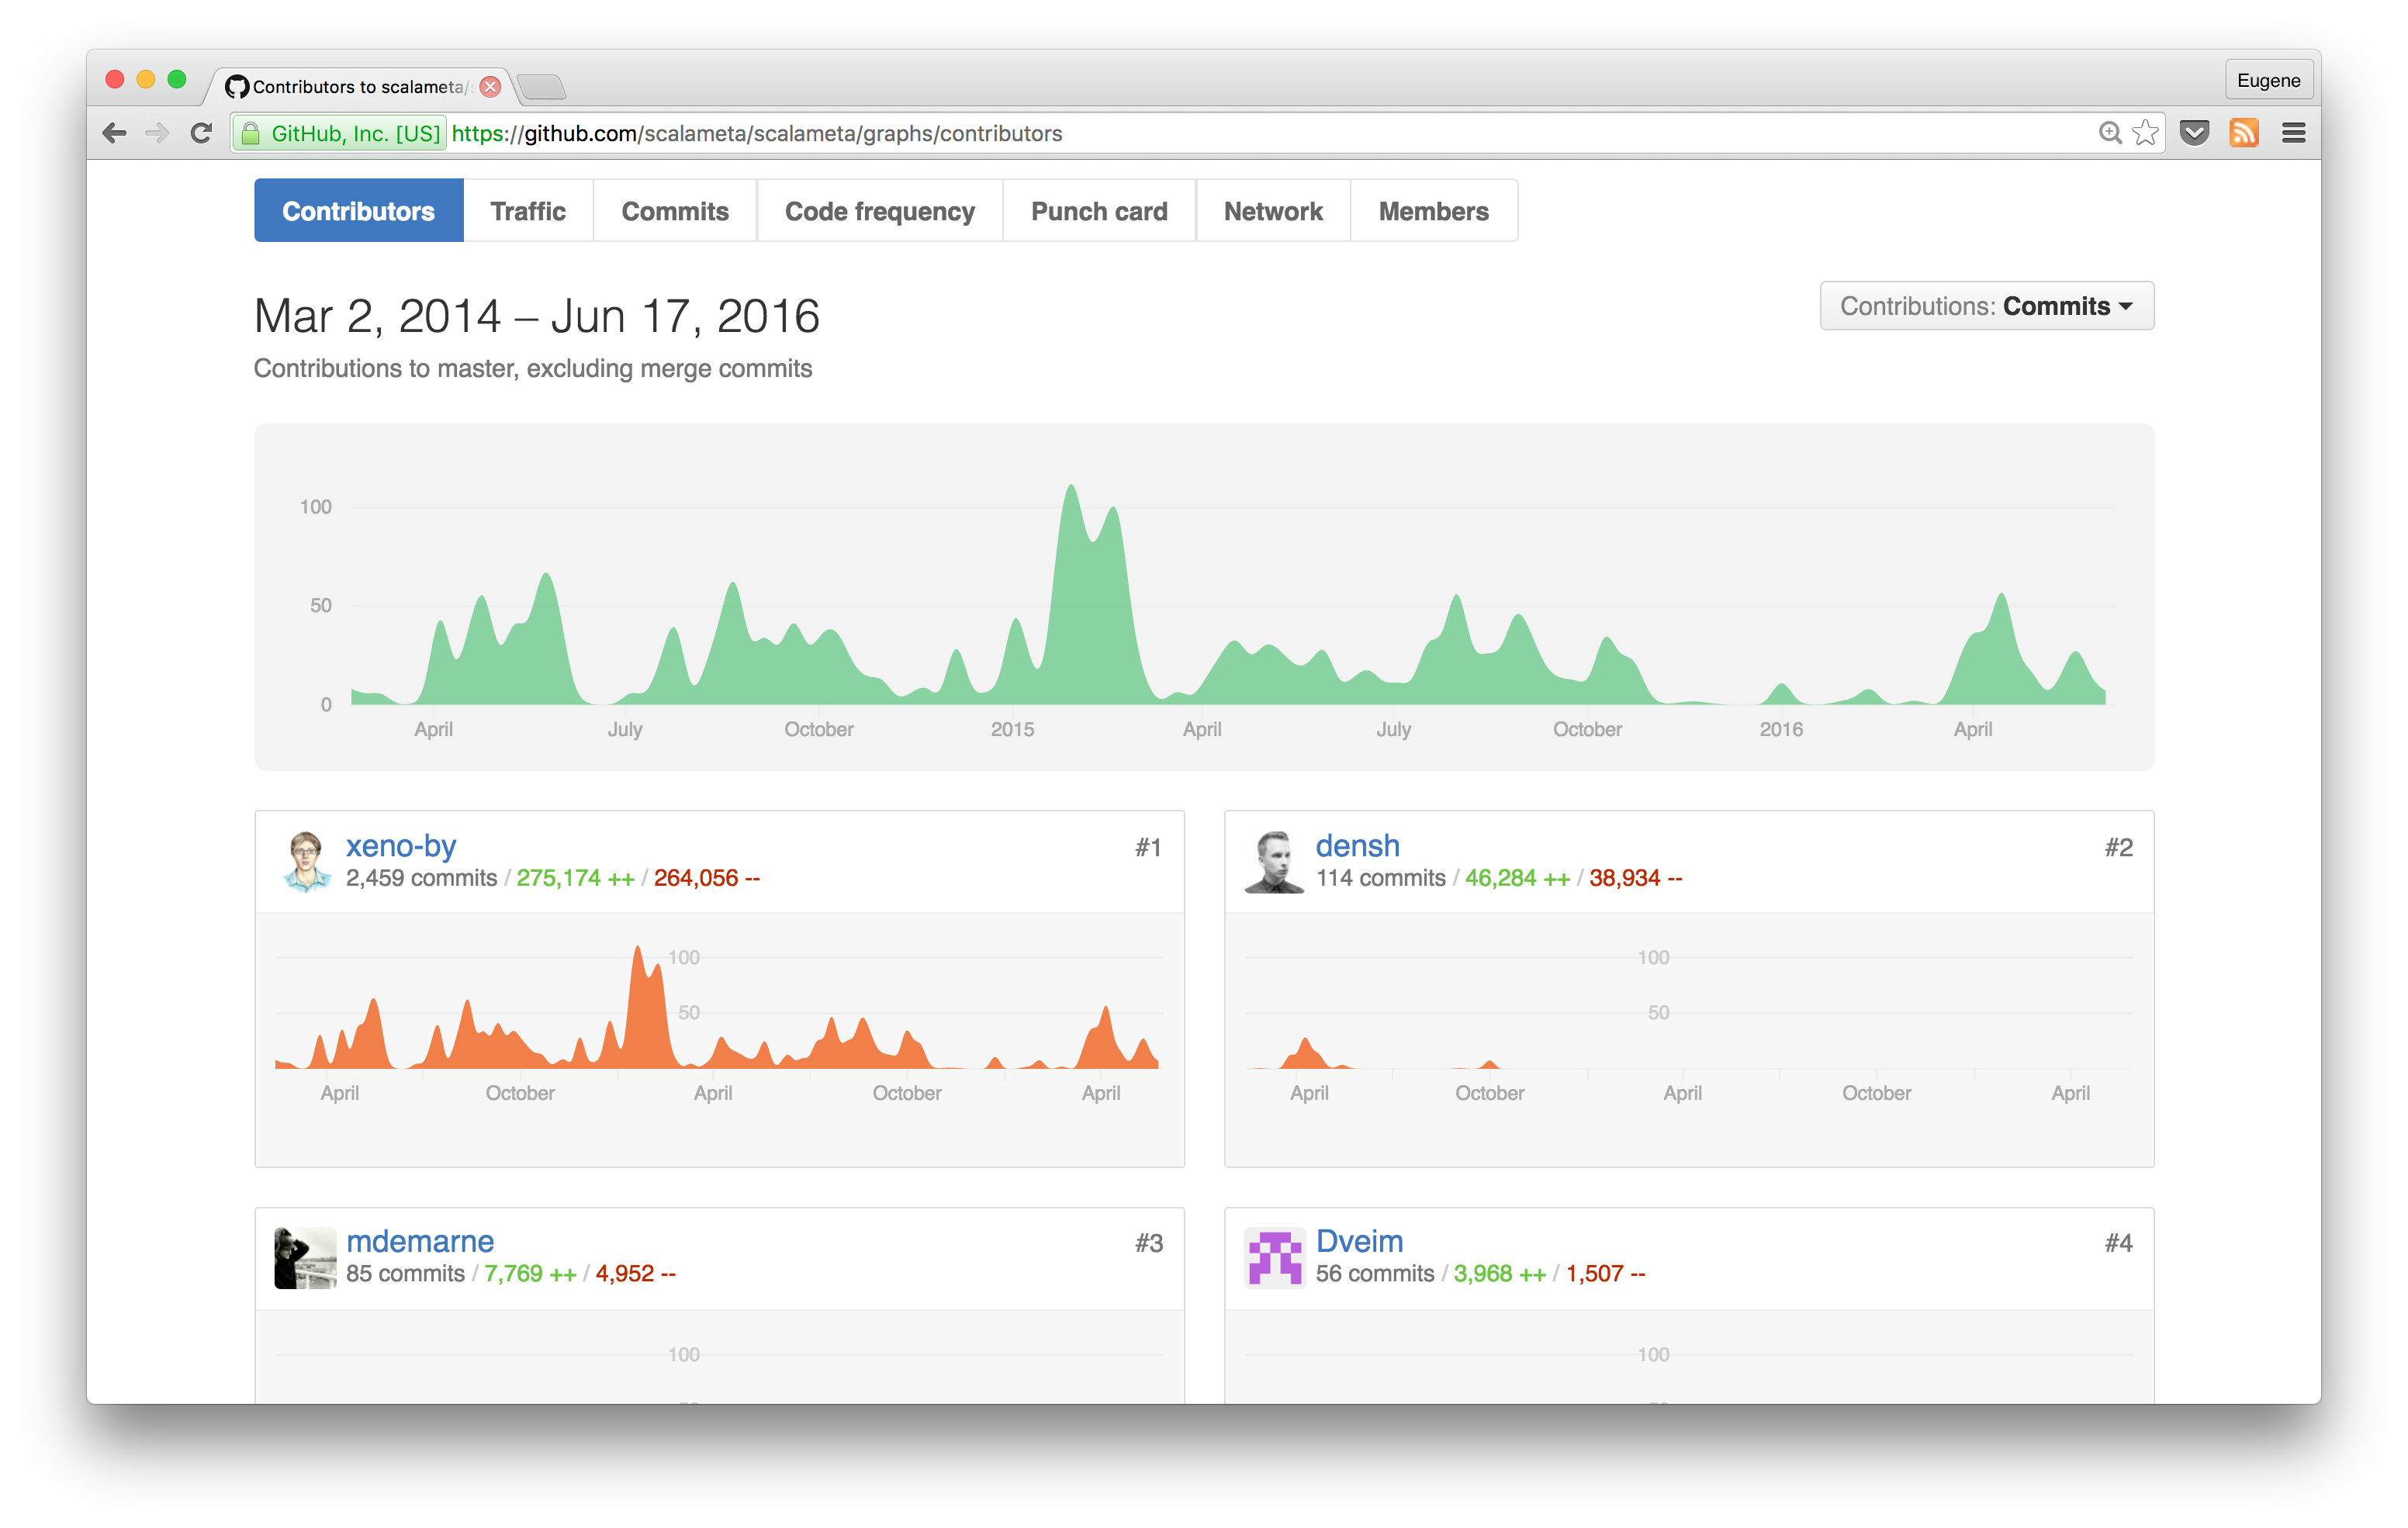
\includegraphics[height=7.75cm]{is-an-active-project.png}
% \end{center}
% \end{frame}

% \begin{frame}{scala.meta is a welcoming community}
\begin{frame}{scala.meta is an active project}
\begin{center}
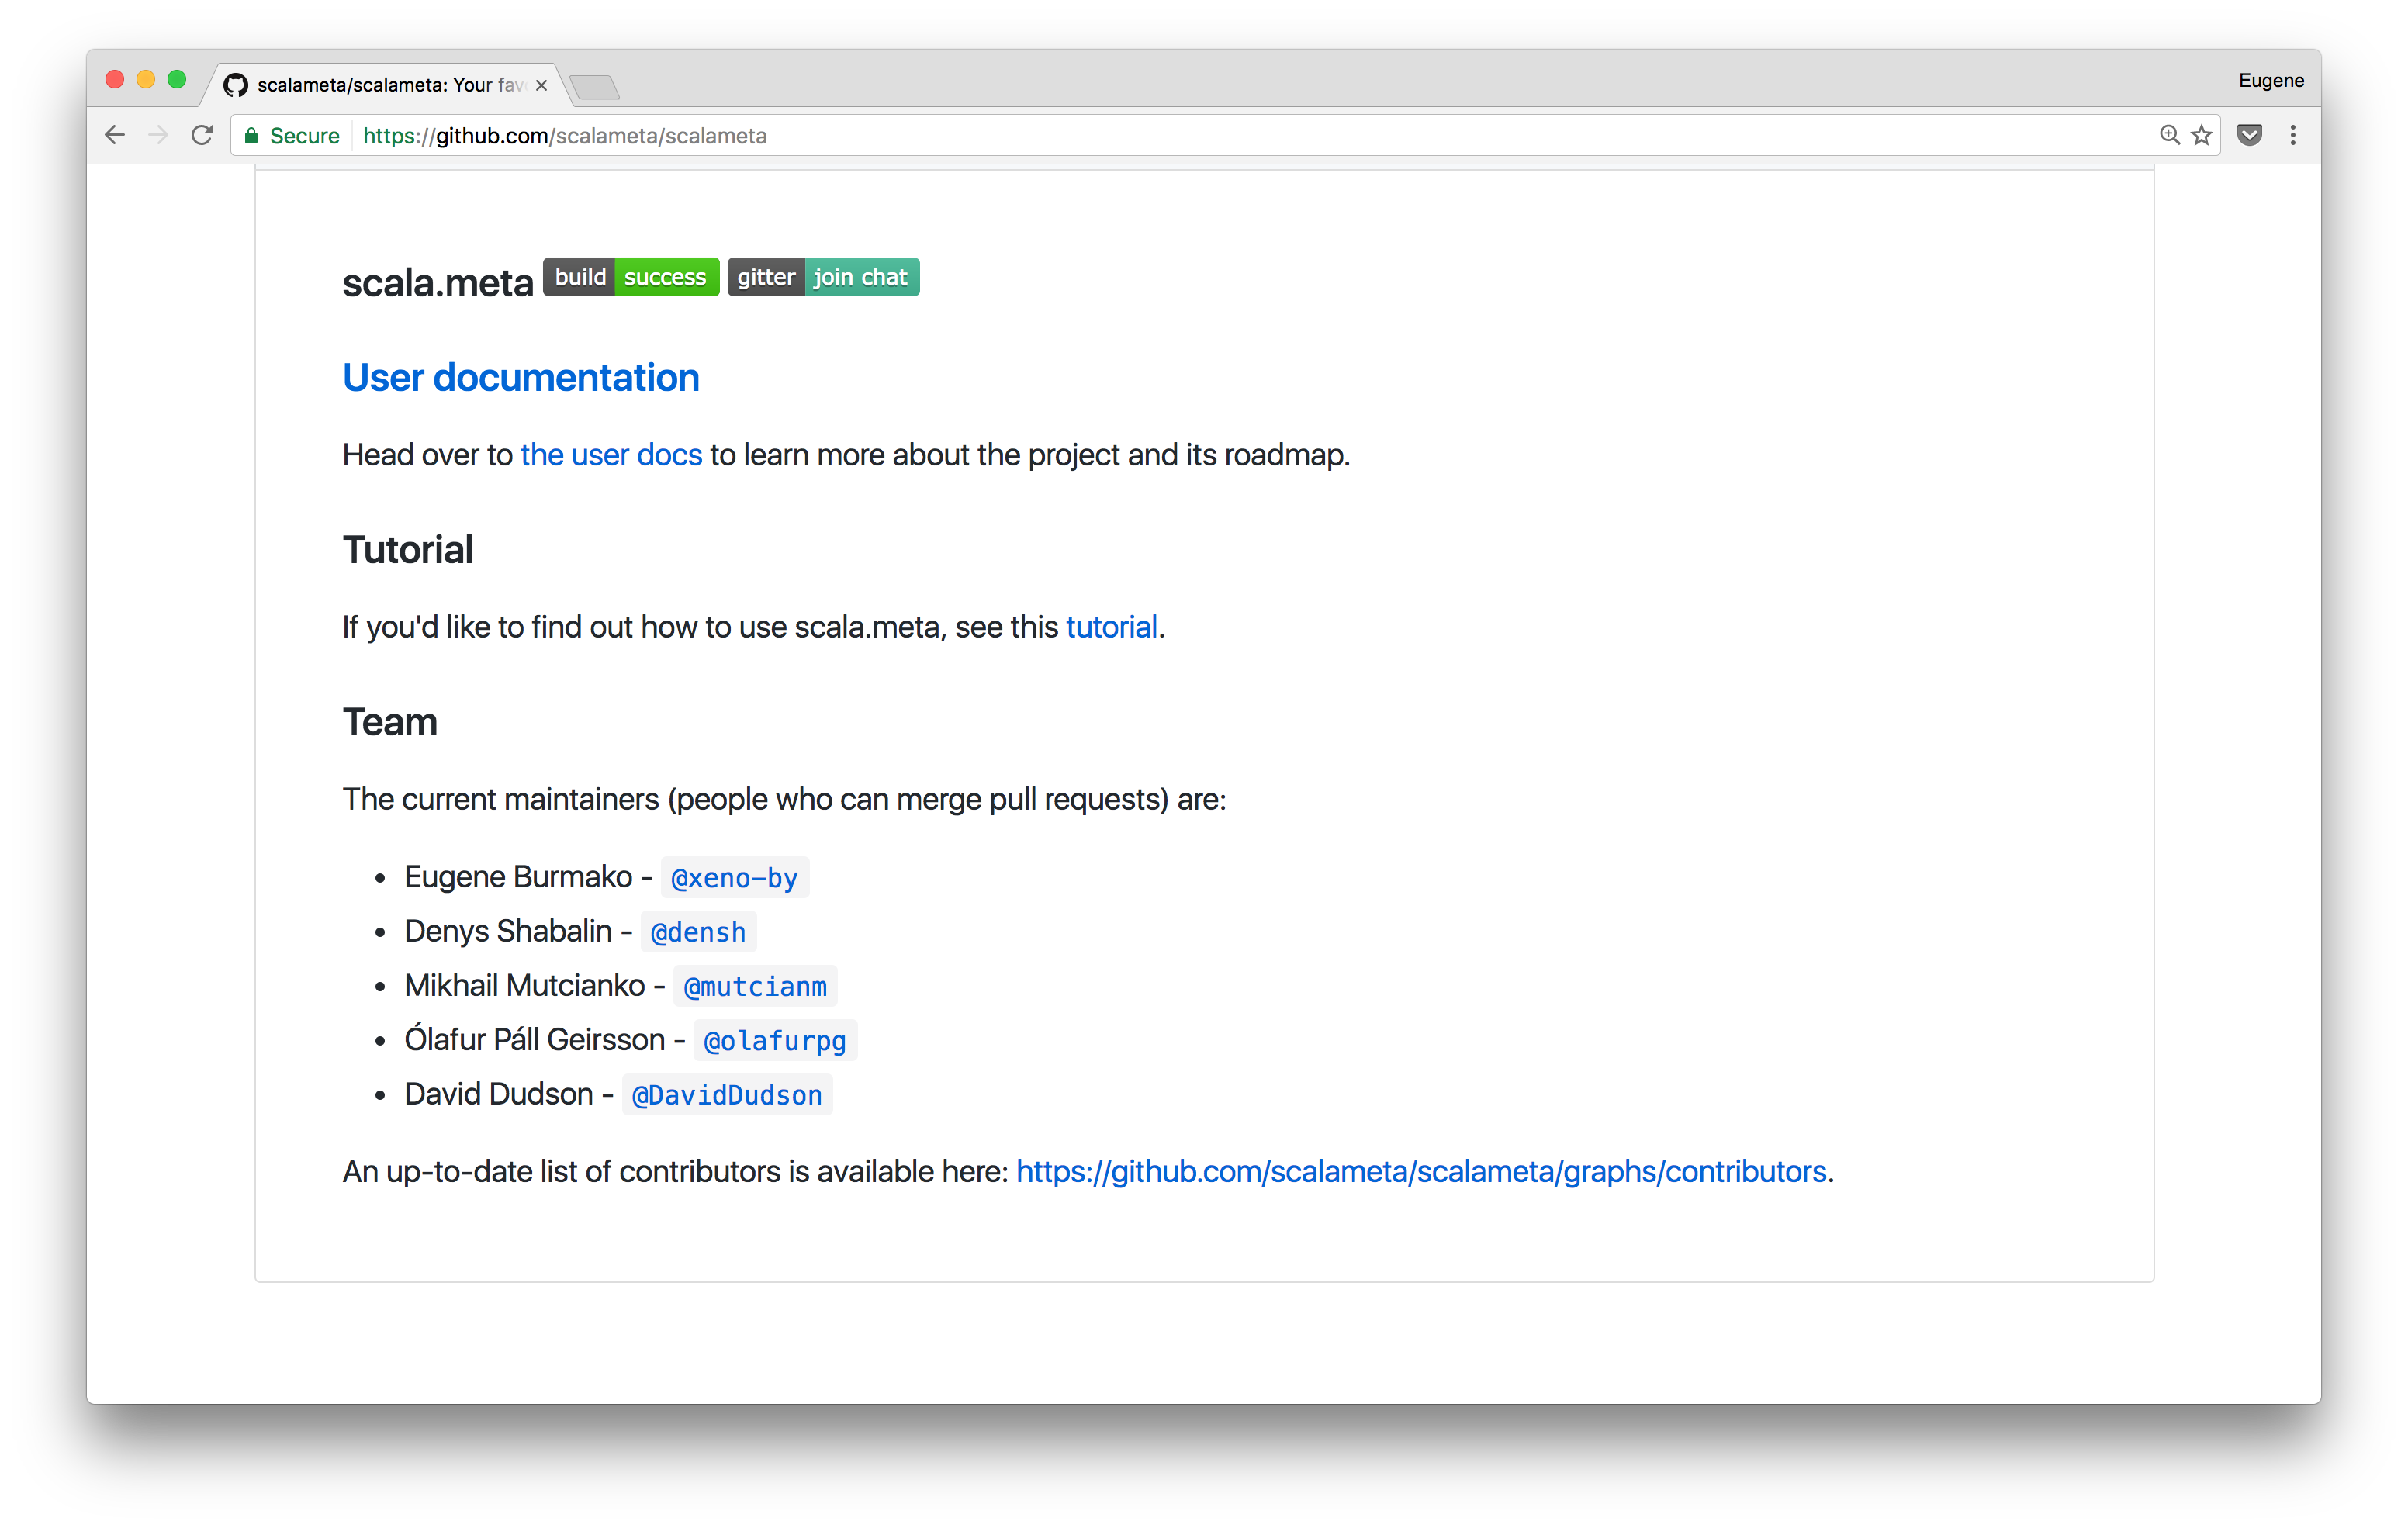
\includegraphics[height=7.75cm]{is-a-welcoming-community.png}
\end{center}
\end{frame}

\sectionframe{Scala.meta API}

\begin{frame}[fragile]{Syntactic API}
\begin{semiverbatim}
scala> import scala.meta._
import scala.meta._

scala> "println(List(1, 2, 3))".parse[Term].get
res0: scala.meta.Term = println(List(1, 2, 3))

scala> res0.structure
res1: String = Term.Apply(
  Term.Name("println"),
  Seq(Term.Apply(
    Term.Name("List"),
    Seq(Lit(1), Lit(2), Lit(3)))))

scala> res0.tokens
res2: scala.meta.tokens.Tokens =
Tokens(, println, (, List, (, 1, ,,  , 2, ,,  , 3, ), ), )
\end{semiverbatim}
\end{frame}

\begin{frame}{Semantic API}
\begin{itemize}
\item \alert<2>{What does a name resolve to?}
\item \alert<3>{What type does an expression have?}
\item \alert<4>{What does an expression desugar to?}
\end{itemize}

\vskip25pt
\only<2>{
\begin{semiverbatim}println(List(1, 2, 3))\end{semiverbatim}
\begin{itemize}
\item \texttt{println} resolves to \texttt{scala.Predef.println}
\item \texttt{List} resolves to \texttt{scala.List}
\end{itemize}
}
\only<3>{
\begin{semiverbatim}println(List(1, 2, 3))\end{semiverbatim}
\begin{itemize}
\item \texttt{println} has type \texttt{(Any)Unit}
\item \texttt{List} has type \texttt{List.type}
\item \texttt{1}, \texttt{2} and \texttt{3} have type \texttt{Int}
\item \texttt{List(1, 2, 3)} has type \texttt{List}
\item \texttt{println(List(1, 2, 3))} has type \texttt{Unit}
\end{itemize}
}
\only<4>{
\begin{semiverbatim}println(List(1, 2, 3))\end{semiverbatim}
\begin{itemize}
\item \texttt{List(...)} desugars to \texttt{List.apply(...)}
\item \texttt{List.apply(...)} desugars to \texttt{List.apply[Int](...)}
\end{itemize}
}
\end{frame}

\begin{frame}{Our research shows that...}
\begin{itemize}
\item These three questions can be easily answered using compiler internals
\item Answering them robustly and portably is very hard
\item Comprehensive solutions most likely require person-years to implement
\item ...and maintain
\end{itemize}
\end{frame}

\begin{frame}{Rethinking our strategy}
\begin{itemize}
\item Incrementally ship semantic APIs in bite-sized portions
\item Implementation simplicity trumps comprehensiveness
\item Portability is still a fundamental goal of the project
\end{itemize}
\end{frame}

\begin{frame}[fragile]{In this talk}
\begin{semiverbatim}
scala> q"println(List(1, 2, 3))"
res0: scala.meta.Term = println(List(1, 2, 3))

scala> res0.structure
res1: String = Term.Apply(
  \alert{Term.Name("println")},
  Seq(Term.Apply(
    \alert{Term.Name("List")},
    Seq(Lit(1), Lit(2), Lit(3)))))
\end{semiverbatim}
\end{frame}

\sectionframe{Semantic databases}

\begin{frame}{Semantic databases}
\begin{center}
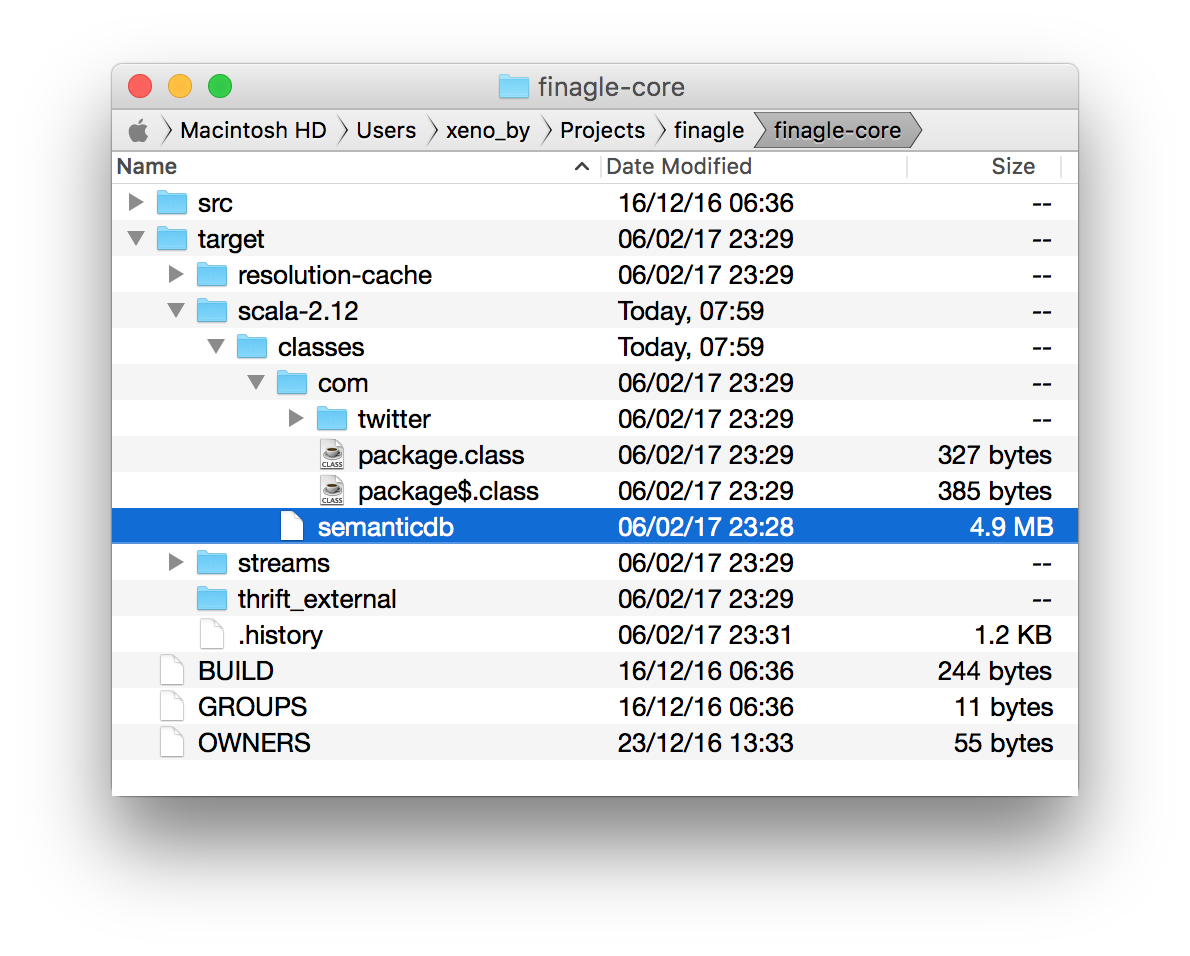
\includegraphics[height=9cm]{semantic-db.png}
\end{center}
\end{frame}

\begin{frame}[fragile]{Semantic databases}
\begin{semiverbatim}
$ ls
Library.scala

$ cat Library.scala
object Library \{
  def main(args: Array[String]): Unit = \{
    println(List(1, 2, 3))
  \}
\}
\end{semiverbatim}
\end{frame}

\begin{frame}[fragile]{Semantic databases}
\begin{semiverbatim}
$ scalac -Xplugin:.../scalahost.jar -Yrangepos Library.scala

$ ls
Library$.class
Library.class
Library.scala
semanticdb
\end{semiverbatim}
\end{frame}

\begin{frame}[fragile]{Semantic databases}
\fontsize{9}{11}\selectfont
\begin{semiverbatim}
$ cat semanticdb
file:/Users/xeno_by/Projects/Meta1x/sandbox/Library.scala
[7..14): Library => _empty_.Library.
[23..27): main => _empty_.Library.main([Ljava/lang/String;)V.
[28..32): args => _empty_.Library.main([Ljava/lang/String;)V.(args)
[34..39): Array => _root_.scala.Array#
[40..46): String => _root_.scala.Predef.String#
[50..54): Unit => _root_.scala.Unit#
[63..70): println => _root_.scala.Predef.println(Ljava/lang/Object;)V.
[71..75): List => _root_.scala.collection.immutable.List.apply(...
\end{semiverbatim}
\end{frame}

\begin{frame}{Discussion}
Semantic databases are...
\begin{itemize}
\item Portable
\item Persistent
\item Distributable
\end{itemize}
\end{frame}

\sectionframe{Mirrors}

\begin{frame}[fragile]{Mirrors}
\begin{semiverbatim}
package scala.meta
package semantic
package v1

trait Mirror \{
  def dialect: Dialect
  def sources: Seq[Source]
  def database: Database
  def symbol(ref: Ref): Completed[Symbol]
\}
\end{semiverbatim}
\end{frame}

\begin{frame}[fragile]{Mirrors}
\begin{semiverbatim}
import scala.meta._

object Test extends App \{
  val classpath = "..."
  val sourcepath = "..."
  implicit val mirror = Mirror(classpath, sourcepath)

  println(mirror.database)

  mirror.sources.foreach \{ source =>
    source.collect \{
      case name @ Term.Name("println") =>
        println(name.symbol)
    \}
  \}
\}
\end{semiverbatim}
\end{frame}

\begin{frame}{Discussion}
You can create a mirror from:
\begin{itemize}
\item An instance of \texttt{scala.tools.nsc.Global}
\item A classpath and a sourcepath
\item An SBT build
\end{itemize}

\vskip15pt
Check out \text{\color{blue}\href{https://github.com/scalameta/sbt-semantic-example}{https://github.com/scalameta/sbt-semantic-example}}
for a complete example and an accompanying guide.
\end{frame}

\sectionframe{Implementation details}

\begin{frame}{Challenges}
\begin{itemize}
\item Attributed trees have platform-dependent representation
\item Including undocumented type inference
\item Including undocumented desugarings
\end{itemize}
\end{frame}

\begin{frame}{Strategy \#1 (2015)}
\begin{itemize}
\item Take compiler ASTs
\item Try to revert platform-dependent desugarings
\item Convert compiler ASTs to platform-independent ASTs
\end{itemize}
\vskip15pt
Half a year of work by compiler experts,
several thousand lines of code,
heavy modifications of the typechecker,
almost works.
\end{frame}

\begin{frame}{Strategy \#2 (2016)}
\begin{itemize}
\item Take compiler attributed ASTs
\item Take platform-independent unattributed ASTs
\item Traverse them together
\item Produce platform-independent attributed ASTs
\end{itemize}
\vskip15pt
Several months of work by compiler experts,
several thousand lines of code,
no modifications to the typechecker,
barely works.
\end{frame}

\begin{frame}{Strategy \#3 (2017)}
\begin{itemize}
\item Take compiler ASTs
\item For every name, locate a corresponding AST
\item For every located AST, obtain and persist its symbol
\item No platform-independent ASTs involved!
\end{itemize}
\vskip15pt
A month of work by compiler experts,
several hundred lines of code,
moderate modifications to the typechecker,
almost works.
\end{frame}

\sectionframe{Future work}

\begin{frame}{Next-generation tools}
\begin{itemize}
\item Def macros
\item Automatic refactorings (scalafix)
\item Intelligent code browsers
\item Better code review tools
\item ...
\end{itemize}
\end{frame}

\begin{frame}{More semantic APIs}
\begin{itemize}
\item \texttt{Symbol.tpe}, \texttt{Symbol.members} and friends
\item \texttt{Type.=:=}, \texttt{Type.<:<} and friends
\item Additional functionality, strictly on per-usecase basis
\end{itemize}

\vskip15pt
Check out \text{\color{blue}\href{https://github.com/scalameta/scalameta/issues/604}{https://github.com/scalameta/scalameta/issues/604}}
for the current roadmap and links to individual work items.
\end{frame}

\begin{frame}{Richer semantic databases}
\begin{itemize}
\item Support for types
\item Maybe even desugarings
\item Tool-specific information (e.g. unused imports for scalafix)
\end{itemize}
\end{frame}

\sectionframe{Summary}

\begin{frame}{Summary}
\begin{itemize}
\item Scala.meta 1.6.0 ships with v1 of the semantic API
\item Currently, the semantic API only includes \texttt{Ref.symbol}
\item But we plan to iteratively ship more and more functionality in 2017
\item This work is based on semantic databases - a major innovation in itself
\end{itemize}
\end{frame}

\begin{frame}{Call for contributions}
We need help with testing our semantic database technology.
See \text{\color{blue}\href{https://github.com/scalameta/sbt-semantic-example}{https://github.com/scalameta/sbt-semantic-example}}
for details.

\vskip15pt
To learn more:
\begin{itemize}
\item Ping us on Gitter: \text{\color{blue}\href{https://gitter.im/scalameta/scalameta}{https://gitter.im/scalameta/scalameta}}
\item Find me at a discussion table tomorrow at 12:00
\item Join the scala.meta hackathon tomorrow at 17:00
\item Attend our Scala Days talks in Chicago and Copenhagen
\end{itemize}
\end{frame}

% mention hackathon, maybe in intro

\end{document}